\documentclass[xcolor=dvipsnames, handout]{beamer}
\usetheme{Hannover}
\usecolortheme[named=ForestGreen]{structure}

\setbeamertemplate{sidebar right}{}
\setbeamertemplate{footline}{%
\hfill\usebeamertemplate***{navigation symbols}
\hspace{0.5cm}\insertframenumber{}/\inserttotalframenumber}

\title[BECiECC]{Binary Edwards Curves in Elliptic Curve Cryptography}
\author{Graham Enos}
\institute[UNCC Math]{UNC Charlotte Department of Mathematics and Statistics}
\date[Mar 29, 2013]{Dissertation Defense, March 29, 2013}

\begin{document}

\frame{\titlepage}

\begin{frame}
    \frametitle{Outline}
    \tableofcontents[pausesection]
\end{frame}

\section{Introduction}

\begin{frame}
    \frametitle{Motivation}
    Edwards curves are extremely useful for cryptography; they offer better
    safety from the ground up.\\
    Less work has been done on binary Edwards curves.
\end{frame}

\begin{frame}
    \frametitle{Contributions}
    In this dissertation, we
    \begin{enumerate}
        \pause
        \item show that binary Edwards curves are safer than some other
            recently proposed normal forms
        \pause
        \item calculate pairings on binary Edwards curves
        \pause
        \item give two new cryptographic applications of binary Edwards curves
        \pause
        \item construct \texttt{e2c2}, a modern C++11 library for Edwards
            elliptic curve cryptography
    \end{enumerate}
    \pause
    First: some background on elliptic curves, cryptography, and Edwards curves
\end{frame}

\section{Elliptic Curves and Cryptography}

\begin{frame}
    \frametitle{Elliptic Curves and Cryptography}
    In the 80s, Koblitz and Miller proposed using the group of points on an
        elliptic curve as the basis for public key cryptography.
    \begin{itemize}
        \item They offer strong security for much smaller key sizes.
        \item They have a nice geometric description of the group law.
        \end{itemize}   
\end{frame}

\begin{frame}
    \frametitle{Weierstrass Group Law}
    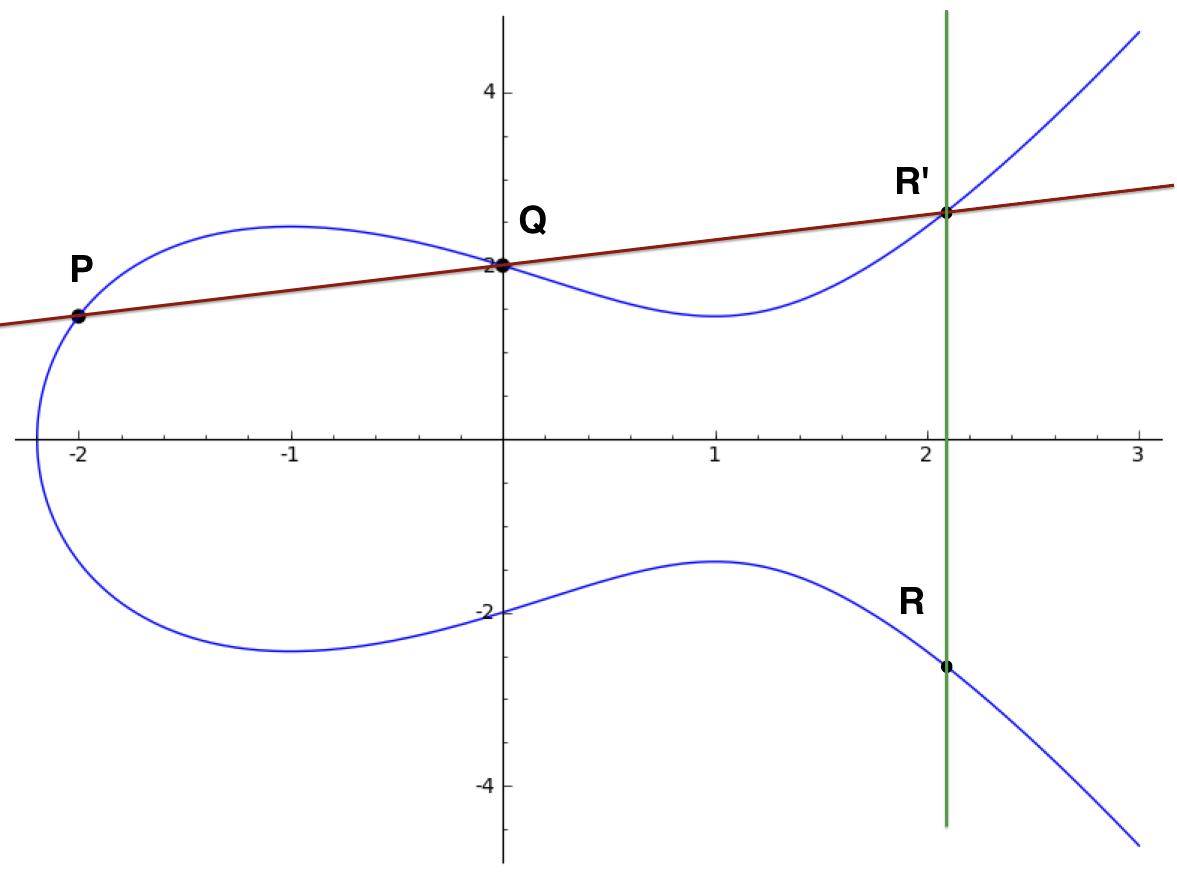
\includegraphics[scale=.5]{wgl.png}
\end{frame}

\begin{frame}
    \frametitle{Side-Channel Worries}
    However, there are some issues\dots
    \begin{itemize}
        \pause
        \item What if $P = \infty$? What if $Q = \infty$?
        \pause
        \item What if $P = Q$?
        \pause
        \item What if $P.x = Q.x = 0$?
        \pause
        \item What if $P = -Q$?
        \pause
    \end{itemize}
    \alert{The group law has to check for all of these.}
\end{frame}

\begin{frame}
    \frametitle{Edwards Curves}
    Edwards gave a new normal form in 2007, which was then extended by
        Bernstein and Lange:
    \begin{displaymath}
        E_{O, c, d}: \quad x^2 + y^2 = c^2(1 + dx^2y^2)
    \end{displaymath}
        such that $cd(1 - dc^4) \ne 0$.
\end{frame}

\begin{frame}
    \frametitle{Edwards Curves}
    \begin{center}
    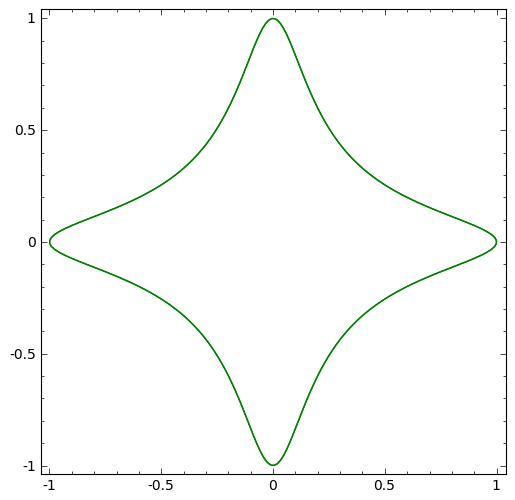
\includegraphics[scale=.5]{ec1.png}
    \end{center}
\end{frame}

\begin{frame}
    \frametitle{Edwards ECC}
    Complete and unified group law
    \begin{enumerate}
        \pause
        \item[$\implies$] No special cases (doubling, identity element, etc.)
        \pause
        \item[$\implies$] Less prone to side-channel attacks
        \pause
        \item[$\therefore$] Safer from the ground up
    \end{enumerate}
\end{frame}

\begin{frame}
    \frametitle{Twisted Edward Curves}
    These are quadratic twists of Edwards curves, cover more cases; more work
        is done with them nowadays.\\
    \alert{Their group law is also unified and complete.}
\end{frame}

\section{Binary Edwards Curves}

\begin{frame}
    \frametitle{Characteristic Two}
    Those were only defined over fields of characteristic $\ne 2$.
    Characteristic 2 is nice from an implementation standpoint.
    Bernstein et.al. to the rescue!
\end{frame}

\begin{frame}
    \frametitle{Binary Edwards Curves}
    \begin{displaymath}
        E_{B, d_1, d_2}: \quad d_1(x + y) + d_2(x^2 + y^2) = xy(x + 1)(y + 1)
    \end{displaymath}
    If the field's defining polynomial has degree $\ge 3$, all binary elliptic
        curves are birationally equivalent \alert{over the base field} to a
        complete binary Edwards curve.
\end{frame}

\begin{frame}
    \frametitle{Binary Edwards Group Law}
    $(x_1, y_1) + (x_2, y_2) = (x_3, y_3)$ where
    \begin{align*}
        x_3 =  &\frac{N_x}{D_x}\\
        y_3 =  &\frac{N_y}{D_y}\\
        N_x =  &d_1(x_1 + x_2) + d_2(x_1 + y_1)(x_2 + y_2) +\\
               &(x_1 + x_1^2)(x_2(y_1 + y_2 + 1) + y_1y_2)\\
        D_x =  &d_1 + (x_1 + x_1^2)(x_2 + y_2)\\
        N_y =  &d_1(y_1 + y_2) + d_2(x_1 + y_1)(x_2 + y_2) +\\
               &(y_1 + y_1^2)(y_2(x_1 + x_2 + 1) + x_1x_2)\\
        D_y =  &d_1 + (y_1 + y_1^2)(x_2 + y_2)
    \end{align*}
    \pause
    \alert{complete and unified}
\end{frame}

\section{Practical Considerations}

\begin{frame}
    \frametitle{New Normal Forms}
    More normal forms have been recently proposed claiming unified and complete
    group laws.\\
    \pause
    Most of them are, but only modulo the ideal generated by the curve
        equation.\\
    \pause
    All three types of Edwards have a simple neutral element and a symmetric
        group law; no need to reduce modulo an ideal.
\end{frame}

\begin{frame}
    \frametitle{Farashahi \& Joye}
    \begin{displaymath}
    \mathbf{H}_{c, d}:\quad X^3 + Y^3 + cZ^3 = dXYZ
    \end{displaymath}
    Suppose we let $P = (X_1 : Y_1 : Z_1)$ and $Q = (X_2 : Y_2 : Z_2)$
\end{frame}

\begin{frame}
    \frametitle{Farashahi \& Joye}
    $P + Q = (X_3 : Y_3 : Z_3)$, where
    \begin{align*}
        X_3 &=  cY_2Z_1^2Z_2 - X_1X_2^2Y_1\\
        Y_3 &=  X_2Y_1^2Y_2 - cX_1Z_1Z_2^2\\
        Z_3 &=  X_1^2X_2Z_2 - Y_1Y_2^2Z_1
    \end{align*}
    \pause
    but $Q + P = (X_4 : Y_4 : Z_4)$, such that
    \begin{align*}
        X_4 &=  cY_1Z_1Z_2^2 - X_1^2X_2Y_2\\
        Y_4 &=  X_1Y_1Y_2^2 - cX_2Z_1^2Z_2\\
        Z_4 &=  X_1X_2^2Z_1 - Y_1^2Y_2Z_2
    \end{align*}
    \pause
    \alert{Asymmetry of group law $\implies$ need to reduce modulo the equation
        for $\mathbf{H}_{c, d}$}
\end{frame}

\begin{frame}
    \frametitle{Wang, Tang, \& Yang}
    \begin{displaymath}
        \widetilde{M_d}:\quad X^2Y + XY^2 + dXYZ + Z^3 = 0
    \end{displaymath}
    \pause
    \alert{Arithmetic is quite flawed\dots}
\end{frame}

\begin{frame}
    \frametitle{Wu, Tang, \& Feng}
    \begin{displaymath}
        X^2Y + XY^2 + tXYZ + XZ^2 + YZ^2 = 0
    \end{displaymath}
    Neutral element: $\mathcal{O} = (1 : 1 : 0)$\\
    \pause
    \alert{Unusual choice of neutral element $\implies$ need to reduce modulo
        curve equation to see that $P + \mathcal{O} = P$}
\end{frame}

\begin{frame}
    \frametitle{Diao \& Fouotsa}
    \begin{displaymath}
        \mathcal{E}_\lambda: 1 + x^2 + y^2 + x^2y^2 = \lambda xy
    \end{displaymath}
    \pause
    Addition:
    \begin{displaymath}
        (x_1, y_1) + (x_2, y_2) = \left(
            \frac{x_1 + y_1x_2y_2}{y_2 + x_1y_1x_2},
            \frac{x_1x_2 + y_1y_2}{1 + x_1x_2y_1y_2}
        \right)
    \end{displaymath}
    while
    \begin{displaymath}
        (x_2, y_2) + (x_1, y_1) = \left(
            \frac{x_2 + x_1y_1y_2}{y_1 + x_1x_2y_2},
            \frac{x_1x_2 + y_1y_2}{1 + x_1x_2y_1y_2}
        \right)
    \end{displaymath}
    \pause
    \alert{asymmetric group law}\\
    \pause
    \textbf{Binary Edwards curves are still king!}
\end{frame}

\section{Pairings}

\begin{frame}
    \frametitle{Pairings and Cryptography}
    Pairings are bilinear forms over elliptic curves.\\
    They've proven useful in cryptography, e.g. ``MOV attack'' and
        ``Boneh-Franklin ID-based encryption.''\\
    Some work's been done on pairings for twisted Edwards curves, but not
        binary.\\
    \pause
    \alert{Their calculation hinges on finding a \textit{Miller function} $f$
        with appropriate divisor $div_P(f) = n(P) - n(\mathcal{O})$.}
\end{frame}

\begin{frame}
    \frametitle{Following Das \& Sarkar}
    Idea: map from $E_{B, d_1, d_2}$ to a Weierstrass curve, compute the
    pairing there, then map back
    \pause
    \begin{theorem}
        Let $P_1, P_2 \in E_{B, d_1, d_2}$ such that $P_1 + P_2 = P_3$; then
        the Miller function $h(x, y)$ such that 
        \begin{displaymath}
            div(h) = (P_1) + (P_2) - (P_3) - \mathcal{O}
        \end{displaymath}
        is given by $\frac{N}{D}$, where
    \end{theorem}
    \begin{displaymath}
    D =
        (u1 + u2)
        (u_{3}  d_{1}  (d_{1} X Z + d_{1} Y Z + X Y) + \sqrt{a_6}  Z  (X + Y))
    \end{displaymath}
\end{frame}

\begin{frame}
    \frametitle{Das \& Sarkar, continued}
    $P_1 \ne P_2 \implies$
    \begin{align*}
        N   &= Z  (X + Y)  d_{1}^{2}  (v_{1} u_{2} + u_{1} v_{2} + u_{1}
                \sqrt{a_6} + u_{2}\sqrt{a_6})\\
            &+ \sqrt{a_6}  (u_{1} + u_{2})  d_{1}  (X Y + X Z + Y Z)\\
            &+ Y  X  d_{1}  (v_{1} u_{2} + u_{1} v_{2})\\
            &+ \sqrt{a_6} (X Z u_{1} b + Y Z u_{1} b + X Z u_{2} b + Y Z u_{2}
                b\\
            &+ X Y u_{1} + X Z u_{1} + X Z v_{1} + Y Z v_{1} + X Y u_{2} + X Z
                u_{2} \\
            &+ X Z v_{2} + Y Z v_{2})
    \end{align*}
    $P_1 = P_2 \implies$
    \begin{align*}
    N   &= u_{1}  Z  (X + Y)  d_{1}^{2}  (u_{1}^{2} + \sqrt{a_6})\\
        &+ u_{1}  d_{1}  (X Y u_{1}^{2} + X Y \sqrt{a_6} + X Z \sqrt{a_6} + Y Z
            \sqrt{a_6})\\
        &+  \sqrt{a_6}  (X Z u_{1}^{2} + Y Z u_{1}^{2} + X Z u_{1} b + Y Z
                u_{1} b\\
        &+ X Y u_{1} + X Z u_{1} + X Z v_{1} + Y Z v_{1})
    \end{align*}
\end{frame}

\begin{frame}
    \frametitle{Directions for Future Work}
    Ar\`ene et.al. gave a new geometric interpretation of the twisted group law
        $\implies$ calculation of pairings on $E_{T, a, d}$ directly.\\
    We'd like to do the same for $E_{B, d_1, d_2}$, but the geometry is
        different\dots\\
    We give a theorem that's (hopefully) a step in the right direction.
\end{frame}

\begin{frame}
    \frametitle{Following Ar\`ene et.al.}
    \begin{theorem}
    Let $P_1, P_2 \in E_{B, d_1, d_2}(K)$ be two affine, not
        necessarily distinct, points.
    Let $C$ be the conic passing through $\Omega_1, \Omega_2,
        \mathcal{O}^\prime, P_1,$ and $P_2$ which must have the form
    \begin{displaymath}
        c_{XY}(XY + Z^2) + c_{XZ}(XZ + Z^2) + c_{YZ}(YZ + Z^2)
    \end{displaymath}
    (If some of the above points are equal, we consider $C$ and $E_{B, d_1,
        d_2}$ to intersect with at least that multiplicity at the corresponding
        point.)
    Then the coefficients of the conic $C$ are uniquely determined (up to
        scalars) as follows:
\end{theorem}
\end{frame}

\begin{frame}
    \frametitle{Ar\`ene et.al., continued}
    \begin{enumerate}
        \item
        $P_1 \ne P_2, P_1 \ne \mathcal{O}^\prime, P_2 \ne \mathcal{O}^\prime
            \implies$
        \begin{align*}
            c_{XY}  &=Z_1Z_2\left[X_1(Y_2 + Z_2) + Y_1(X_2 +Z_2) + Z_1(X_2 +
                Y_2)\right]\\
            c_{XZ}  &=Y_1Z_2(X_1Y_2 + X_1Z_2 + Z_1Z_2)\\
                    &+ Y_2Z_1(Y_1X_1 + Z_1X_1 + Z_1Z_2)\\
            c_{YZ}  &=X_1Z_2(Y_1X_2 + Y_1Z_2 + Z_1Z_1)\\
                    &+ X_2Z_1(X_1Y_2 + Z_1Y_2 + Z_1Z_2)
        \end{align*}
        \item
        $P_1 \ne P_2 = \mathcal{O}^\prime \implies c_{XY} = Z_1, c_{XZ} =
            Z_1, c_{YZ} = X_1$
        \item
        $P_1 = P_2 \implies$
        \begin{align*}
            c_{XY}  &=  X_1^2Y_1 + X_1Y_1^2 + d_1X_1Z_1^2 + X_1^2Z_1 +
                d_1Y_1Z_1^2\\
                    &+ Y_1^2Z_1 + X_1Z_1^2 + Y_1Z_1^2\\
            c_{XZ}  &=  X_1^2Y_1 + d_1Y_1^2Z_1 + X_1Y_1^2 + d_1X_1Z_1^2 +
                X_1^2Z_1\\
                    &+ d_1Y_1Z_1^2 + X_1Y_1Z_1 + d_1Z_1^3 + Y_1Z_1^2\\
            c_{YZ}  &=  d_1X_1^2Z_1 +d_2X_1^2Z_1 + d_2Y_1^2Z_1 + X_1^2Z_1 +
                d_1Z_1^3 + X_1Z_1^2
        \end{align*}
    \end{enumerate}
\end{frame}

\section{Applications}

\begin{frame}
    \frametitle{$E_{B, d_1, d_2}$ in Cryptography}
    We offer two applications of binary Edwards curves:
    \begin{enumerate}
        \item \texttt{ECOH's Echo}, a PBKDF
        \item A compartmented id-based secret sharing scheme with
        un/signcryption
    \end{enumerate}
\end{frame}

\begin{frame}
    \frametitle{\texttt{ECOH's Echo}}
    This is a scalable PBKDF, for which we can increase computation time as
        computers get faster.\\
    We modify \texttt{ECOH}, entrant to the SHA-3 competition.\\
    Fixing its main issue, a second preimage attack, in turn leads to
        resistance to parallelization.\\
    We build up $Q$ from input, taking into account output of each previous
        step.
\end{frame}

\begin{frame}
    \frametitle{\texttt{ECOH's Echo}, First Round}
    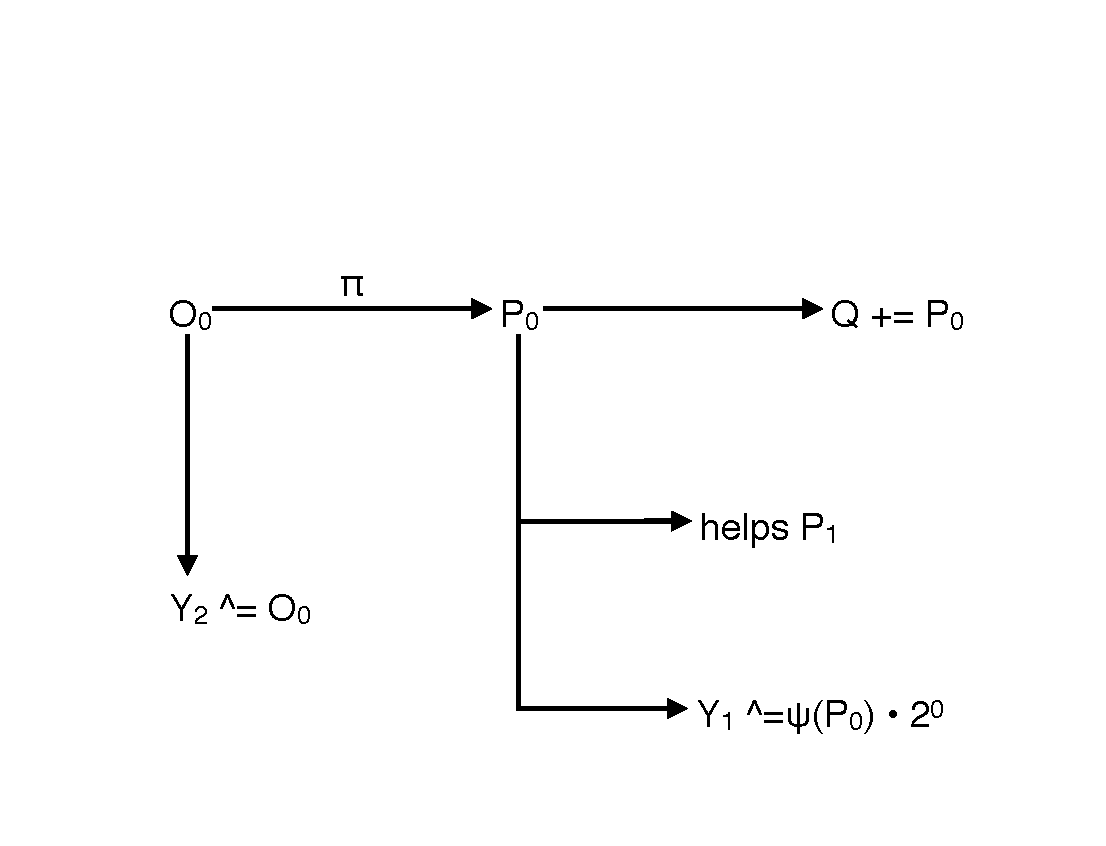
\includegraphics[scale=0.5]{ecoh_echo.pdf}
\end{frame}

\begin{frame}
    \frametitle{\texttt{ECOH's Echo}, Subsequent Rounds}
    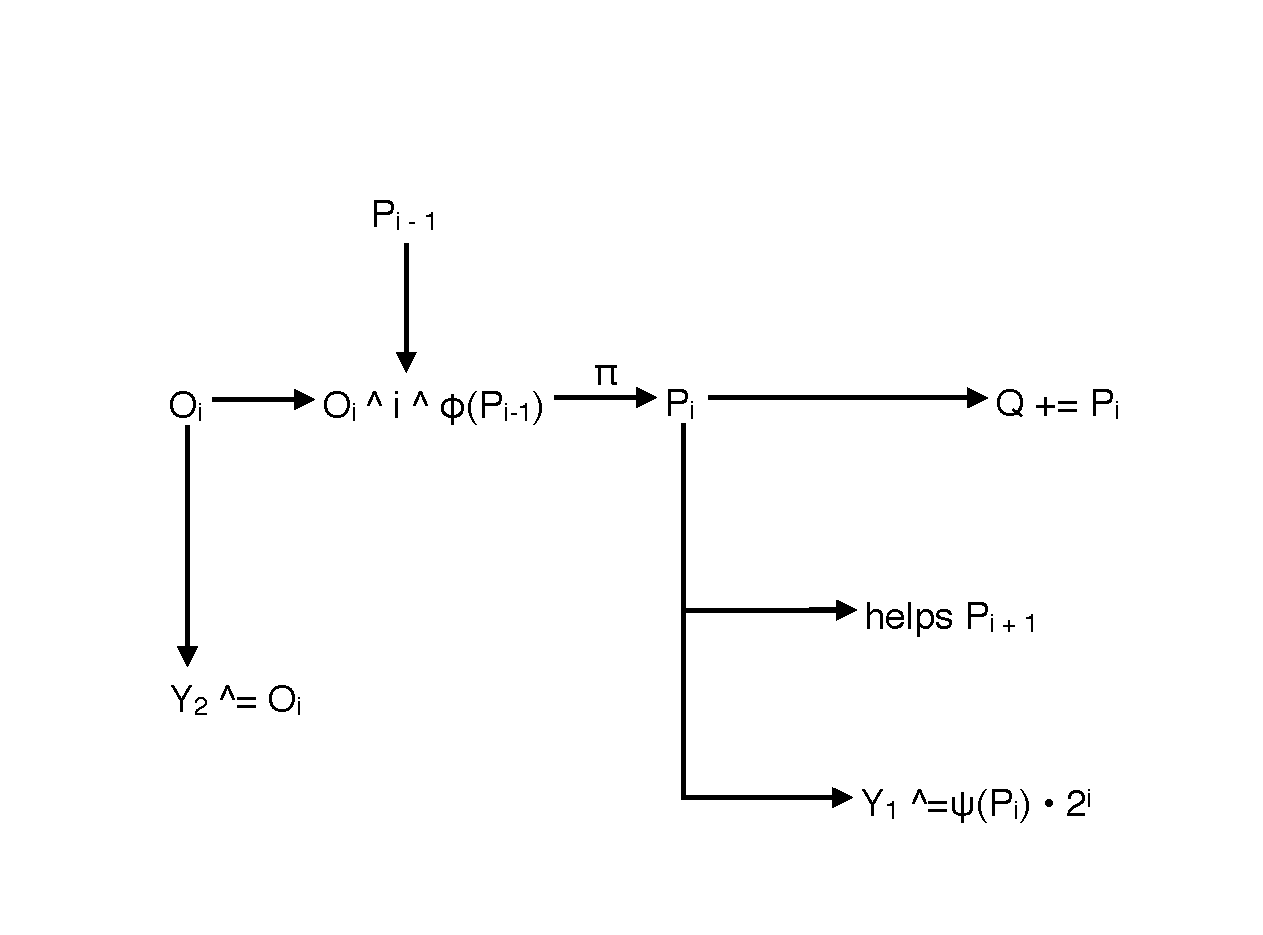
\includegraphics[scale=0.5]{ecoh_echo2.pdf}
\end{frame}

\begin{frame}
    \frametitle{\texttt{ECOH's Echo}, Finish}
    Finally,
    \begin{align*}
        X_1 &\gets \pi(Y_1)\\
        X_2 &\gets \pi\left(Y_1 \oplus Y_2\right)\\
        Q &\gets Q + X_1 + X_2
    \end{align*}
    Return $\varphi(Q)$
\end{frame}

\begin{frame}
    \frametitle{Compartmented ID-Based Secret Sharing and Signcryption}
    My scheme extends a \textit{secret sharing} (send a message to $n$ entities
        in such a way that $t$ of them must cooperate to put it back together)
        to a \textit{compartmented scheme} (send a message to an organization
        broken into $t$ compartments, one representative of each must
        cooperate).\\
    \pause
    It involves \textit{signcryption} so each compartment can verify the
        cooperation of the others and the signature of the original sender.\\
    \pause
    Its cryptography is based on pairings.
\end{frame}

\section{\texttt{e2c2}: a C++11 library}

\begin{frame}
    \frametitle{\texttt{e2c2}}
    In order to explore the theory and implementation of Edwards curves for
        elliptic curve cryptography, I've created a modern C++11 software
        library called \texttt{e2c2}.\\
    It tries to bridge the gap between ``proof-of-concept'' and
        ``production-ready.''\\
    It's certainly not ready for cryptographic primetime, but it gets quite
        decent speed, even on my puny laptop, and the security afforded by the
        simplicity of implementing Edwards curves is very advantageous.
\end{frame}

\begin{frame}
    \frametitle{Interlude}
    \texttt{e2c2} demonstration
\end{frame}

\section{Conclusion}

\begin{frame}
    \frametitle{Contributions}
    To sum up, we saw
    \begin{enumerate}
        \item that binary Edwards curves are safer than some other
            recently proposed normal forms
        \item how to calculate pairings on binary Edwards curves
        \item (a glimpse of) two new cryptographic applications of binary
        Edwards curves
        \item a demonstration of \texttt{e2c2}, a modern C++11 library for
            Edwards elliptic curve cryptography
    \end{enumerate}
\end{frame}

\begin{frame}
    \frametitle{Publication Hopes}
    I'm pursuing publication of some of this work
    \begin{enumerate}
    \item Chapter 4 is online \texttt{http://eprint.iacr.org/2013/015}, and has
        been submitted to \textit{IACR's CRYPTO2013} conference
    \item I'm in the process of revising a paper on the compartmented sharing
    scheme per reviewers' comments from the \textit{Information Processing
    Letters}; see \texttt{http://eprint.iacr.org/2012/528} for a previous
    version
    \item Recently a password hashing contest has been announced, see
    \texttt{https://password-hashing.net/}, and Dr. Zheng and I are hoping to
    submit \texttt{ECOH's Echo}
    \end{enumerate}
\end{frame}

\begin{frame}
    \frametitle{Thanks}
    Many thanks to Dr. Zheng, Dr. Hetyei, rest of my defense committee, UNCC
        Math Department.
\end{frame}

\begin{frame}
    \frametitle{Questions}
    Any questions?
\end{frame}

\end{document}
